\section{Introduction}
\subsection{The Ripstik}
A caster board, known commercially as a RipStik, is a two-wheeled, human powered vehicle.
The board is similar to a skateboard; however, it features two platforms, each with a wheel connected to a free spinning caster.
These platforms are connected by a torsion bar. 
This gives the caster board rider the unique ability to generate propulsion without removing their feet from the board through a series of small turns. 
This configuration also allows for tighter turn and more responsive speed control when compared to a skateboard. 
These characteristics could make the Ripstik a practical vehicle for the urban commuter.
\begin{figure}[!htb]
\centering
\minipage{0.5\textwidth}
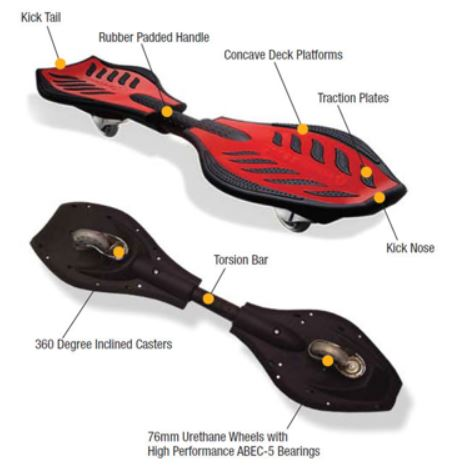
\includegraphics[width=\linewidth]{Ripstik.JPG}
\caption{Detailed description of the components of a Ripstik \cite{PIC}}\label{fig:Ripstik}
\endminipage
\end{figure}
\par
A significant inhibitor to widespread Ripstik adoption is developing competency in riding the board. 
As part of the Ripstik’s design, a unique, full-body movement is required to generate the necessary forces for propulsion. 
For most new riders, this technique requires significant practice in order to develop the ability to ride a Ripstik safely with confidence. 
Developing an electronic control system for the vehicle could facilitate riding, reducing the learning curve associated with the board while preserving the advantages of the Ripstik. 
However, a Ripstik is a sophisticated mechanical system and will require complex mathematical modeling to understand and represent all forces present in the system at a given time.

The addition of a control system to a caster board presents the potential for significant conflicts. 
Aside from the challenges associated with the development of the mathematical model and control system, issues pertaining to the patents for a caster board \cite{casterboardPatent} and restricted operation of the device \cite{TOLaws} may represent a barrier in bringing the product to market. 
Additionally, a mechanical system will be required to execute the commands of the control system. 
The difficulties associated with the recycling of batteries \cite{BatteryRecharge}, housing \cite{PlasticAssessment} and motors may threaten the environmental feasibility of the final design. 
The system may also be susceptible to "hacking" by outside sources \cite{DEFCON}, which could pose a significant safety risk to the operator. 
If these issues are addressed and mitigated, the potential of the device to minimize injuries associated with riding caster boards and to serve as a viable alternative to motor vehicles can be realized. 
This product has the potential to redefine urban commuting across the world by introducing a safe, cost-effective and environmentally-friendly option for short distance travel. 


\subsection{Technical Background} \label{introMath}
\subsubsection{Lagrangian Mechanics}
Lagrangian mechanics will be utilized to accurately model the dynamics of the caster board rather than classical Newtonian mechanics. 
In a complex system with multiple boundary conditions, the Lagrangian method can be used to eliminate forces of constraint \cite{LagrangePowerpoint}. 
A secondary advantage of Lagrangian mechanics lies in the ability to arrive at the same sets of equations from different coordinate systems \cite{LagrangePowerpoint}. 

The Lagrangian function can be represented by L, and is defined as the difference between kinetic and potential energies modeled using positions and velocities \cite{NonholonomicPowerpoint}. 
In the equation, T represents the kinetic energy and V represents the potential energy.

The mathematical formulation for the Lagrangian can be seen in equation [1]: 
\begin{equation}
L=T-V
\end{equation}
\subsubsection{The Euler-Lagrange Equation}
Given the Lagrangian for a system, the goal is to extremize the action integral. 
Simply put, if the path of the system is changed while fixing the endpoints, the variation in the action should be kept to a minimum. 
The variation in the action will be represented by $\vartheta(s,t)$. 
More notably, a curve in $C^2(q_a,q_b,[a,b])$ is an extremal for the action $A_L$ when it satisfies the Euler-Lagrange equations \cite{Lewis}. 
In the provided context, $q_a$ and $q_b$ are coordinates in any defined system on the interval [a,b]. 
Any curve $\gamma$ $\in$ $C^2(q_a,q_b,[a,b])$ that minimizes $A_L$ and satisfies the Euler-Lagrange equations also satisfies the following equation \cite{Lewis}:

\begin{equation} \label{ELeq1}
\frac{d}{ds}\Big|_{s=0}\int_a^b L(t,\frac{d}{dt}\vartheta (s,t))dt
\end{equation}
The equations of motion are developed through the Euler-Lagrange equation. A mathematical representation can be seen in equation \ref{ELeq1}:
\begin{equation}
\frac{d}{dt}(\frac{\partial L}{\partial \dot{q}_{{i}}})-\frac{\partial L}{\partial q_{i}}
\end{equation}

The trajectory of the system is defined by the Euler-Lagrange equation and is based on a set of initial conditions \cite{NonholonomicPowerpoint}. 
The Euler-Lagrange equation is equivalent to Newton's second law \cite{NonholonomicPowerpoint}, and are implicit second-order differential equations when placed into a coordinate system \cite{Lewis}.
\subsubsection{Euler Angles}
Euler angles can be used to describe the orientation of a rigid body. Euler angles are simply described as three rotations around a reference frame axis \cite{EulerAnglesPowerpoint}. 
An example of three angles that can be created by the rotations are the yaw, pitch, and roll \cite{EulerAnglesPowerpoint}.
\par
With the Euler angles defined, a rotation matrix can then be created.  One must first define a standard basis in $\mathbb{R}^3$ by \{$e_1$, $e_2$, $e_3$\}. The mapping will be \cite{Lewis}:
\par
\begin{center}
\par
Eul: $(\pi,\pi]\times(-\frac{\pi}{2},\frac{\pi}{2})\times(-\pi,\pi] \rightarrow \{R\in SO(3)| R_{31}\neq \pm 1\}$
\end{center}
\par

shown by
\par
\begin{equation}
(\alpha, \psi, \theta) \mapsto \exp(\alpha\hat{e_3})\exp(\psi\hat{e_2})\exp(\theta\hat{e_1})
\end{equation}
This produces the following rotation matrix:

\begin{equation} R =
\begin{bmatrix} 
\cos\alpha\cos\psi & \cos\alpha\sin\psi\sin\theta - \cos\theta\sin\alpha &\cos\alpha\cos\theta\sin\psi+\sin\alpha\sin\theta\\
\cos\psi\sin\alpha & \cos\alpha\cos\theta+\sin\alpha\sin\psi\sin\theta & \cos\theta\sin\alpha\sin\psi - \cos\alpha\sin\theta\\
 -\sin\psi & \cos\psi\sin\theta & \cos\psi\cos\theta 
\end{bmatrix}
\end{equation}
\par
The rotation matrix R can be used to describe the rotation from the body-fixed frame to the inertial frame \cite{VTOL}.

\subsubsection{Nonholonomic Constraints}
Once the number of degrees of freedom for the system are developed, the nonholonomic constraints can be well defined. 
Nonholonomic constraints must be expressed by the differentials of the coordinates, are non-integrable, and restrict the velocities of the system \cite{LagrangeEquations}. 
The nonholonomic constraints can be mathematically represented through the following equations:

\begin{equation}
\sum_{i=1}^{n}a_{ji}dq_i+a_{jt}dt=0, j=1,...,m
\end{equation}
Where n is the number of coordinates of the system, represented by $q_i$, i=\{1,...,n\}, and m is the number of constraint equations. The $t$ term represents the time dimension. 
\begin{equation}
a_{ji}=f(q_1,...,q_n,t)
\end{equation}
In the nonholonomic equation, $a_{ji}$ are coefficients for each coordinate and time.

A differential equation is said to be integrable (holonomic) if the equations are exact. For i,k=1,...,n; j=1,...,m \cite{LagrangeEquations}:
\begin{equation}
\frac{\partial{a_{ji}}}{\partial{q_{k}}}= \frac{\partial{a_{jk}}}{\partial{q_{i}}}
\end{equation}
\begin{equation}
\frac{\partial{a_{ji}}}{\partial{t}}= \frac{\partial{a_{jt}}}{\partial{q_{i}}}
\end{equation}
Careful application of the preceding principles should lead to a comprehensive and accurate mathematical model of the system.